\documentclass[10pt]{beamer}

\usetheme[nosectionslide]{m}

% camel case
\renewcommand{\mthemetitleformat}{}

\definecolor{mDarkRed}{HTML}{8F0129}
\definecolor{mGreen}{HTML}{0E8740}
\setbeamercolor{alerted text}{fg=mGreen}
\setbeamertemplate{bibliography item}[text]

\setbeamertemplate{footnote}{\hangpara{2em}{1}\makebox[2em][l]{\insertfootnotemark}\footnotesize\insertfootnotetext\par}


\usepackage[scale=2]{ccicons}

\usepackage{cmap}           % Mapeamento de caracteres especiais no PDF
\usepackage{lmodern}        % Usa fonte Latin Modern
\usepackage[T1]{fontenc}    % Seleção de codificação de fonte
\usepackage[utf8]{inputenc} % Codificação do arquivo (conversão automática dos acentos)
\usepackage[brazil]{babel}  % Idioma para hifenização e tradução de vários elementos
\usepackage{makeidx}        % Criação de índice
\usepackage{hyperref}       % Formatação do índice
\usepackage{lastpage}       % Usado pela Ficha catalográfica
\usepackage{indentfirst}    % Indenta o primeiro parágrafo de cada seção
% \usepackage[usenames,dvipsnames]{xcolor}  % Controle das cores (com nomes)
\usepackage{graphicx}       % Inclusão de gráficos
\usepackage{booktabs}       % Formatação de tabelas
% -------------------------------------------------------------------------------------------------
% Para citações
\usepackage[brazilian,hyperpageref]{backref} % Páginas com as citações na bibliografia
\usepackage[alf]{abntex2cite} % Citações padrão ABNT (alfanumérico)
% -------------------------------------------------------------------------------------------------
% Pacotes opcionais
\usepackage{nomencl}        % Para criar uma lista de símbolos
\usepackage{acro}           % Para usar acrônimos e abreviaturas
\usepackage{tikz}           % Para fazer figuras, diagramas e gráficos integrados e elegantes
\usepackage{pgfplots}       % Usa o pacote tikz para fazer gráficos muito melhores que os do Excel
\usepackage{pgfplotstable}  % Para gerar tabelas automaticamente a partir de arquivos com dados
\usepackage{filecontents}   % Para colocar o conteúdo de um arquivo dentro de um arquivo tex
\usepackage{todonotes}      % Para criar anotações durante o desenvolvimento do texto
%\usepackage{multirow}       % Permite fazer tabelas com múltiplas linhas
\let\newfloat=\undefined    % Workaround para usar o pacote algorithm
\usepackage{algorithm}      % Para escrever algoritmos
\usepackage{algpseudocode}
\usepackage{pifont}
% \usepackage{clrscode}       % Para escrever algoritmos
% \usepackage{clrscode3e}     % Para escrever algoritmos; mais simples que os pacotes acima
\usepackage{pdfpages}        % Para incluir a folha de aprovação assinada em PDF
\usepackage{amsmath}
\usepackage{amsfonts}
\usepackage{subcaption}
\newcolumntype{P}[1]{>{\centering\arraybackslash}m{#1}} 

\usepackage{tablefootnote}
\usepackage{adjustbox}

\captionsetup{labelformat=empty,labelsep=none}


\makeatletter
\newcommand\footnoteref[1]{\protected@xdef\@thefnmark{\ref{#1}}\@footnotemark}
\makeatother

\DeclareMathOperator*{\argmin}{arg\,min}
\DeclareMathOperator*{\argmax}{arg\,max}


\title{Aprendizagem Guiada para Análise Morfossintática usando Redes Neurais Recursivas}
\subtitle{}
\date{8 de julho de 2015}
\author[Treviso]{Marcos Vinícius Treviso\\\scriptsize\texttt{ marcosvtreviso@gmail.com}\\\\Orientador: Fábio Natanael Kepler\\}
\institute{Universidade Federal do Pampa}
\titlegraphic{\hfill\includegraphics[height=1.25cm]{img/unipampa_logo.png}}

\begin{document}

\maketitle

\begin{frame}
  \frametitle{Agenda da apresentação}
  \setbeamertemplate{section in toc}[mine]
  \tableofcontents[hideallsubsections]
\end{frame}


\section{Introdução}


\begin{frame}[fragile]
  \frametitle{Introdução}

  \begin{itemize}
      \item \textit{Part-of-speech} (POS) Tagging 
      \item O problema
      \item Objetivos
    \end{itemize}


\end{frame}


\begin{frame}[fragile]
  \frametitle{POS Tagging}

  É conhecido em Processamento de Linguagem Natural (PLN) como o ato de classificar uma palavra pertencente a um conjunto de textos em uma classe gramatical.

 \begin{itemize}
      \item[-] Acurácia
      \item[-] Aplicações
      \item[-] Desafios
    \end{itemize}

  
    \begin{figure}[htb]
    \begin{center}
        \includegraphics[scale=0.5]{img/exemploclassificacao.pdf}
    \end{center}
    % \caption{Exemplo de classificação gramatical}\label{fig:exemploclassificacao}
  \end{figure}

\end{frame}


\begin{frame}[fragile]
  \frametitle{O problema}

  

 \begin{itemize}
      \item[-] Há muita ambiguidade no português 
      \item[-] Estratégia trivial não é eficaz
      \item[-] É necessário analisar o contexto
      \item[-] Aprendizado de máquina
    \end{itemize}

  
    \begin{figure}[htb]
    \begin{center}
        \includegraphics[scale=0.35]{img/funcoes.pdf}
    \end{center}
    % \caption{Função sobrejetora Vs. Função multivalorada}\label{fig:funcoes}
  \end{figure}

\end{frame}



\begin{frame}[fragile]
  \frametitle{Objetivos}


 \begin{itemize}
    \item[-] Novo método para POS Tagging
    \begin{itemize}
      \item[-] A príncipio para o português brasileiro
    \end{itemize}
    \item[\ ] \ 
    \item[-] Estado da arte
    \begin{itemize}
      \item[-] Novas técnicas
      \item[-] Novas abordagens
    \end{itemize}
     \item[\ ] \ 
    \item[-] Análise de eficiência
    \begin{itemize}
      \item[-] Acurácia
      \item[-] Tempo de treinamento
    \end{itemize}
  \end{itemize}

\end{frame}




\section{Fundamentação}

\begin{frame}[fragile]
  \frametitle{Fundamentação}

  \begin{itemize}
    \item Aprendizado de máquina
    \item Córpus
    \item Representação das palavras
    \item Redes neurais
    \item Aprendizagem profunda
  \end{itemize}
  

\end{frame}


\begin{frame}[fragile]
  \frametitle{Aprendizado de máquina}

  \begin{itemize}
    \item[-] Aprendizado supervisionado
    \begin{itemize}
      \item[-] Regressão
      \item[-] Classificação  
    \end{itemize}
    \item[-] Aprendizado não supervisionado
  \end{itemize}

  \begin{figure}[htb]
  \begin{center}
      \includegraphics[scale=0.38]{img/passoapasso.png}
   % \caption{Matriz de coocorrência para criação de palavras vetorizadas} \label{fig:matrizdecoocorrencia}
  \end{center}
\end{figure}

\end{frame}



\begin{frame}[fragile]
  \frametitle{Córpus}

  \begin{itemize}
    \item[-] Coleções de textos agrupados
    \item[-] Anotação gramatical manual
    \item[-] \textit{Córpus} para o português brasileiro:\\ \

    \begin{table}[!htb]
    \footnotesize
    \centering
    \begin{tabular}{lccc}
      \toprule
      \textbf{Córpus} & \textbf{Sentenças}  & \textbf{Palavras}  & \textbf{Classes gramaticais}  \\
      \midrule
      Mac-Morpho original & 53,374 & 1,221,465 & 41  \\
      Mac-Morpho revisado\footnotemark & 49,932 & 945,958   & 26  \\
      Tycho Brahe         & 96,125 & 1,541,654 & 265 \\
      \bottomrule
    \end{tabular}
    % \caption{Dados dos \textit{córpus}} \label{tab:dadoscorpus}
    \end{table}

  \item[\ ] \ 
  \item[-] Por que não combiná-los?
  \item[\ ] \ 
  \end{itemize}


{\scriptsize 1. Revisado em: \cite{fonseca2015evaluating}.}

\end{frame}



\begin{frame}[fragile]
  \frametitle{Representação das palavras}

  \begin{itemize}
    \item[-] Dados de entrada (\textit{features})
    
    \item[\ ] \ 

    \item[-] Vetores reais valorados em um espaço multidimensional (\textit{word embeddings})
    
    \item[\ ] \ 

    \item[-] Mais desempenho de aplicações em PLN e menos engenharia de \textit{features}

    \item[\ ] \ 

    \item[-] Conseguem capturar informações sintáticas e semânticas

    \item[\ ] \ 

    \item[-] Geradas de maneiras diferentes dependendo da técnica utilizada
  \end{itemize}
  


\end{frame}


\begin{frame}[fragile]
  \frametitle{Técnicas para geração de \textit{word embeddings}}
  
   \begin{itemize}
    \item[-] Matriz de coocorrência

    \item[\ ] \ 

    \item[-] \textit{Neural Language Model} (NLM): Através de redes neurais

    \item[\ ] \ 

    \item[-] \textit{Hyperspace Analogue to Language} (HAL): Matriz de coocorrência com um método de decomposição (Escalamento Multidimensional)

    \item[\ ] \ 

    \item[-] Modelação \textit{Skip-Gram} (SG): Previsão de palavras vizinhas num conjunto de tamanho finito.

    \item[\ ] \ 

    \item[-] \textit{Global Vectors} (GloVe): Razão das probabilidades na matriz de coocorrência em relação ao contexto de uma outra palavra do vocabulário.

  \end{itemize}

  \begin{equation}
  W:word \to \mathbb{R}^n \nonumber
  \end{equation}

\end{frame}

\begin{frame}[fragile]
  \frametitle{Técnicas para geração de \textit{word embeddings}}

   \begin{itemize}
    \item[-] Palavras similares estão próximas.
    \item[\ ] \ 
  \end{itemize}

  \begin{figure}[htb]
  \begin{center}
      \includegraphics[scale=0.18]{img/Turian-WordTSNE}
  \end{center}
  \caption{Fonte: \citeonline{turian2010word}}

\end{figure}


\end{frame}





\begin{frame}[fragile]
  \frametitle{Redes neurais}

  \begin{columns}[onlytextwidth]
    \column{0.5\textwidth}
      
      \begin{itemize}
        \item[-] Simulação do cérebro humano
        \item[\ ] \ 
        \item[-] Unidades de ativação: $a_i^{(j)}$
        \item[\ ] \ 
        \item[-] Pesos: $\theta^{(j)}$
        \item[\ ] \ 
        \item[-] Função de ativação: $g(z)$
        \item[\ ] \ 
        \item[-] Parâmetros: $z^{(j+1)} =  \theta^{(j)}a^{(j)}$
      \end{itemize}

    \column{0.5\textwidth}
      
       \begin{figure}[!htb]
        \begin{center}
        \begin{tikzpicture}
        \begin{axis}[
            width=1.0\textwidth,
            scaled ticks=false,
            log ticks with fixed point,
            ymin=0,ymax=1,xmin=-10,xmax=10,domain=-10:10,
            log basis y = 10,
            title={Função sigmoide},
            xlabel=x,
            ylabel=y,
            legend style={draw=none},
            samples=200,
          ]
          \addplot[blue] { 1 / (1 + pow(e, -x))};
        \end{axis}
        \end{tikzpicture}
        \end{center}
        \end{figure}

  \end{columns}
  

\end{frame}


\begin{frame}[fragile]
  \frametitle{Redes neurais}

  - Processo de aprendizagem:

  \begin{figure}
    \begin{center}
      \includegraphics[scale=0.4]{img/redeneuralmulticlass}
    \end{center}
    \caption{Fonte: \citeonline{machinelearningcoursera}}
  \end{figure}
  
\end{frame}


\begin{frame}[fragile]
  \frametitle{Redes neurais}

  - Processo de aprendizagem:

  \begin{figure}
    \begin{center}
      \includegraphics[scale=0.42]{img/backpropagationalg}
    \end{center}
    \caption{Fonte: \citeonline{machinelearningcoursera}}
  \end{figure}
  
\end{frame}



\begin{frame}[fragile]
  \frametitle{Aprendizagem profunda}

  \begin{columns}[onlytextwidth]
    \column{0.45\textwidth}
      
      \begin{itemize}
        \item[-] Muitas tranformações não lineares
        \item[\ ] \ 
        \item[-] Objetivo de aprender automaticamente boas \textit{features}
        \item[\ ] \ 
        \item[-] Crescimento do desempenho computacional
        \item[\ ] \ 
        \item[-] Redes neurais com múltiplas camadas
      \end{itemize}

    \column{0.55\textwidth}
      
      \begin{figure}
      \begin{center}
        \includegraphics[scale=0.24]{img/aprendendodeep2.pdf}
      \end{center}
      \caption{Adaptade de: \citeonline{Bengio-et-al-2015-Book}}
    \end{figure}
       

  \end{columns}
  

\end{frame}







\section{Trabalhos relacionados}

\begin{frame}[fragile]
  \frametitle{Trabalhos relacionados}

  \begin{itemize}

  \item Escopo do português brasileiro

  \item[\ ] \adjustbox{max height=\dimexpr\textheight-5.5cm\relax,max width=\textwidth}{
  \begin{tabular}{llll}
    \toprule
    \textbf{Autores} & \textbf{Modelo}  & \textbf{Representação das palavras}  & \textbf{Córpus} \\
    \midrule
    \citeonline{kepler2005etiquetador} & VLMM & Sequência de caracteres & Tycho Brahe \\
    \citeonline{dos2014training} & Redes neurais profundas  & Vetores (CharWNN) & Tycho Brahe; Mac-Morpho \\
    \citeonline{fonseca2015evaluating} & Redes neurais & Vetores (NLM, HAL, SG) & Tycho Brahe; Mac-Morpho \\
    Este trabalho & Redes neurais recursivas & Vetores Vetores (NLM, SG, GloVe) & Tycho Brahe; Mac-Morpho \\
    \bottomrule
  \end{tabular}
  }

  \item[\ ] \ 
  \item[\ ] \ 

  \item Estado da arte com 97,57\% de acurácia para todas palavras \cite{fonseca2015evaluating}

  \item[\ ] \ 

  \item Estado da arte com 94,34\% de acurácia para palavras fora do vocábulario \cite{fonseca2015evaluating}
  
  \end{itemize}

\end{frame}





\section{Metodologia}


\begin{frame}[fragile]
  \frametitle{Metodologia}

  \begin{itemize}
    \item Representação das palavras
    \item Pontuações para estrutura gramatical
    \item Treinamento
  \end{itemize}
  

\end{frame}


\begin{frame}[fragile]
\frametitle{Representação das palavras}


  \begin{itemize}

    \item[-] Técnicas:
    \begin{itemize}
      \item[-] NLM
      \item[-] SG
      \item[-] GloVe
    \end{itemize}

    \item[\ ] \begin{align} \nonumber 
    w_i \in \omega \to v_i \in \mathbb{R}^d \\
    c_i \in \gamma \to z_i \in \mathbb{R}^d \nonumber 
    \end{align}

    \item[\ ] \ 

    \item[-] Capitalização

    \item[\ ] \ 

    \item[-] Prefixos

  \end{itemize}

\end{frame}



\begin{frame}[fragile]
\frametitle{Pontuações para estrutura gramatical}


  \begin{itemize}

    \item[-] Janela de palavras com tamanho $t$:

    \item[\ ] $V_n = \big\{ v_{n - (t-1)/2}, ..., v_n, ..., v_{{n + (t-1)/2}} \big\} $

    \item[\ ] \ 

    \item[-] Pontuações para estrutura gramatical:

    \item[\ ] $s_c(V_n)$

    \item[\ ] $A_{c,d,e}$

    \item[\ ] \ 

    \item[-] Pontuação final para $w_i^t$ dado $c_1^t$:

    \item[\ ] \begin{equation} 
S(w_1^t, c_1^t) = \sum\limits_{k=1}^{t} \Big( \argmax_{1 \leq i \leq t, i \notin Q} (s_{c_i}(V_i) + A_{c_{i-1}, c_{i}, c_{i+1}}) \Big) \nonumber
\end{equation}



  \end{itemize}

\end{frame}



\begin{frame}[fragile]
\frametitle{Treinamento}
  
  \begin{itemize}

    \item[-] Treinamento supervisionado

    \item[-] Rede neural recursiva

    \item[-] Aprendizagem guiada por palavras mais fáceis \cite{shen2007guided}

    \item[\ ] \

    \begin{figure}[htb]
        \begin{center}
            \includegraphics[scale=0.35]{img/guidedlearning.pdf}
        \end{center}
    \end{figure}


    \item[\ ] \

    \item[-] Composição dos vetores:

    \item[\ ] $v_n = v_n + z_c$ 

  \end{itemize}


\end{frame}



\begin{frame}[fragile]
\frametitle{Treinamento}
\vspace{-2.5em}


  \begin{figure}
      \begin{center}
        \includegraphics[scale=0.15]{img/neuralnetworkfinal_alg2.pdf}
      \end{center}
    \end{figure}

\end{frame}


\begin{frame}[fragile]
\frametitle{Treinamento}
  
  \begin{itemize}

    \item[-] Ajustamentos feitos para maximizar:

    \item[\ ] \begin{equation}
    \sum\limits_{(w_1^t,c_1^t) \in \phi} P(c_1^t|w_1^t,\theta) \nonumber
    \end{equation}

    \item[\ ] \ 

    \item[-] Função de custo:

    \item[\ ] \begin{equation}
    J(\theta) = log\Bigg(\sum\limits_{u_1^t \in \gamma^t} e^{S(w_1^t, u_1^t)} \Bigg) - S(w_1^t, c_1^t) \nonumber
    \end{equation}

    \item[\ ] \ 

    \item[-] Gradiente Descendente, Gradiente Descendente Estocástico, Adagrad, Adadelta, etc. \cite{Bengio-et-al-2015-Book}

  \end{itemize}


\end{frame}





\section{Cronograma}

\begin{frame}[fragile]
  \frametitle{Cronograma}

  A1 - Implementação do modelo neural recursivo

  A2 - Treinamento do modelo

  A3 - Avaliação dos resultados obtidos

  A4 - Escrita da monografia

  \begin{table}[!htb]
  \footnotesize
  \centering
  \begin{tabular}{cccccc}
    \toprule
    & \textbf{Agosto} & \textbf{Setembro}  & \textbf{Outubro}  & \textbf{Novembro} & \textbf{Dezembro}  \\
    \midrule
    \textbf{A1} & X & X & X &   &   \\
    \textbf{A2} &   & X & X & X &   \\
    \textbf{A3} &   &   & X & X & X \\
    \textbf{A4} &   &   &   & X & X \\
    \bottomrule
  \end{tabular}
  \end{table}



\end{frame}



\section{Referências}

\begin{frame}[allowframebreaks,noframenumbering]

  \frametitle{Referências}
  \bibliography{bibliografia,abntex2-modelo-references}

\end{frame}



% \plain{Aprendizagem Guiada para Análise Morfossintática usando Redes Neurais Recursivas \\ {\scriptsize asddas}}

% \plain{Aprendizagem Guiada para Análise Morfossintática usando Redes Neurais Recursivas \\ \ \\ {\normalsize asd}}

\plain{Aprendizagem Guiada para Análise Morfossintática usando Redes Neurais Recursivas \\ \ \\ {\normalsize Marcos Vinícius Treviso} \\ \texttt{\scriptsize marcosvtreviso@gmail.com} \\ \ \\ {\normalsize Orientador: Fábio Natanael Kepler} \\ \ \\ \ \\ \ \\ {\normalsize 8 de julho de 2015} \\ {\scriptsize Universidade Federal do Pampa}}









\begin{frame}[fragile]
  \frametitle{Redes neurais recursivas}

  \begin{itemize}
    \item Grafo computacional parece como uma árvore
  
    \item Aplica-se transformações recursivamente

     % ``Dado um grafo acíclico dirigido, é visitado os nodos em ordem topológica, e recursivamente aplica-se transformações para gerar novas representações a partir de prévias representações já computadas dos nodos filhos''  


    \item Composição da saída com entrada

    \item[\ ] \ 

    \begin{figure}
      \begin{center}
        \includegraphics[scale=0.25]{img/redeneuralrecursiva.pdf}
      \end{center}
    \end{figure}


  \end{itemize}

\end{frame}



\end{document}
